\documentclass[9pt,indentedstyle,preprint]{sigplanconf}
\usepackage[english]{babel}
\usepackage[sort&compress,numbers]{natbib}
\usepackage[pdftex]{graphicx}

\begin{document}

\conferenceinfo{Haskell'08}{080925, Victoria, BC, Canada.} 
\copyrightyear{2008} 
\copyrightdata{[to be supplied]} 

\titlebanner{Draft}        % These are ignored unless
\preprintfooter{Hask08}   % 'preprint' option specified.

\title{Yi}
\subtitle{An Editor in Haskell for Haskell}

\authorinfo{Jean-Philippe Bernardy}
           {Computer Science and Engineering, 
            Chalmers University of Technology
            % and University of Gothenburg
          }
           {bernardy@chalmers.se}

\maketitle

\begin{abstract}
  Yi is a text editor written in Haskell and extensible in Haskell. We take
  advantage of Haskell's expressive power to define embedded DSLs that form the
  foundation of the editor. In turn, these DSLs provide a flexible
  mechanism to create extended versions of the editor. Yi also
  provides some support for editing Haskell code.
\end{abstract}

\category{D.2.3}{Coding Tools and Techniques}{Program editors}

\terms
Design, Languages

\keywords
Editor, Haskell, Functional Programming

\section{Motivation}

All software developers wants to customize and extend their editor. We
spend so much time working with them that we want them to behave
exactly as we wish.  Using Haskell as an extension language is
promising, because it is both general purpose and high-level. This
combination of properties means that extensions and configurations can remain
concise, and still have unrestricted access to external resources, for
example by using available Haskell libraries.

Also, users generally want to experiment with changes without careful study of
the system they tweak, and the well-known safety features of Haskell are useful
in this case. Users can tinker with the editor and rely on the type system to
guide them in writing correct code.

\section{Overview}

Yi is a text editor implemented in Haskell and, more importantly, extensible in
Haskell. It is structured around four embedded DSLs:
\begin{description}
\item[BufferM] A DSL for all buffer-local operations, like insertion
  and deletion of text, and annotation of buffer contents. It
  can be understood as monad that encapsulates the state of one buffer.
\item[EditorM] A DSL for editor-level operations, e.g., opening and closing
  windows and buffers. Operations involving more than one buffer are
  handled at this level too.
\item[YiM] A DSL for IO-level operations. There, one can operate on files,
  processes, etc.  This is the only level where IO can be done.
\item[KeymapM] Key-binding descriptions. The structure of this DSL
  closely follows that of classic parsing-combinator libraries.  The
  semantics are a bit different though: the intention is to map a
  stream of input events to a stream of actions, instead of producing
  a single result. The actions produced are values in any of the above
  DSLs.
\end{description}
Yi also contains user-interface (UI) code for rendering the editor
state, and getting the stream of input events from the user.  Finally,
there is some glue code to tie the knot between all these
components. This glue is the only part that accesses the UI code.

The structure described above is very flexible: there is very low coupling between
layers. One can easily swap out a component for another in the same
category. For example, the user can choose between various UI
components (vty, gtk, cocoa) and key-bindings (emacs, vim).

The various DSLs have composability properties, and this makes them
suitable configure the editor. For instance, a user 
defines a new \textbf{BufferM} action, using the library of functions available
in Yi, and other Haskell libraries. Then, he creates a new
key-binding for it. Using the disjunction operator, this binding can
then be merged with the default bindings (e.g., emacs), as shown 
in figure~\ref{fig:example}.

\begin{figure}
\begin{verbatim}
import Yi
import Yi.Keymap.Emacs as Emacs
import Yi.String (modifyLines)

increaseIndent :: BufferM ()
increaseIndent = do
  r <- getSelectRegionB 
  r' <- unitWiseRegion Line r 
     -- extend the region to full lines
  modifyRegionB (modifyLines (' ':)) r'
     -- prepend each line with a space
                                     
main :: IO ()
main = yi $ defaultConfig {
  defaultKm = 
     -- take the default Emacs keymap...
     Emacs.keymap <|> 
     -- ... and bind the function to 'Ctrl->'
      (ctrl (char '>') ?>>! increaseIndent)
 }
\end{verbatim}
\caption{Configuration file example.}
\label{fig:example}
\end{figure}

We see that Yi is not so much an editor than a rich library for
building editors. Indeed, this is exactly how users create
extended versions of Yi: they create a program {\em from the ground
  up} by combining the higher-order functions and (lazy) data
structures offered in the Yi library. This approach to
configuration was pioneered by \citet{Stewart2007XMonad}.

\section{Editing Haskell code}

Being implemented and extensible in Haskell, it would be natural that
Yi had extensive support for \emph{editing} programs, and in
particular Haskell code.  At the time of writing, we have implemented
this partially. There is a parsing combinator library to describe
syntax of programs; the contents of buffers are parsed incrementally
and the result is made available to the rest of the code.

We take advantage of this infrastructure to provide support for
Haskell: among other things, feedback on parenthesis matching is given
(as shown in figure~\ref{fig:screenshot}), and there is simple support
for auto-indentation.

\begin{figure}
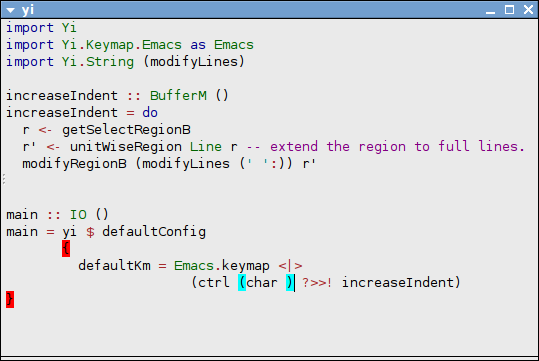
\includegraphics[width=\columnwidth]{screenshot.png}
\caption{Screenshot. The configuration file is being edited, and Yi
  gives feedback on matching parenthesis by changing the background
  color. Yi takes the Haskell layout rule in account: the braces do
  not match because the closing one is not indented.}
\label{fig:screenshot}
\end{figure}

\section{Limitations and Further work}

The parsing mechanism is not perfect yet: we only have a coarse-grained
syntax for Haskell, and the error-correction scheme is lacking
generality.  A further step will be to bind to Haskell compilers, and
in particular GHC, to provide full-fledged IDE capabilities, in the
fashion of Visual Haskell \cite{Angelov2005VH}.

Yi is also lacking dynamic capabilities: while the configuration
mechanism is flexible, activating a new configuration requires {\em
  restarting} the editor.  We plan to solve this problem by saving the
editor state before restart and reloading it afterwards. This approach is
feasible because the state of the editor is a purely functional data
structure.

We point the interested reader to the Yi homepage \cite{YiHome} for
further information, or to download and install Yi from Hackage
\cite{Hackage}.

\acks 

The Yi project was started in 2004 by Don Stewart
\cite{Stewart2005Dynamic}. Yi has had more than forty contributors
since then ---too many to cite individually--- but
they shall all be thanked for sharing the load in pushing Yi
forward. I would like to mention a few of them, though: the early
adopters Allan Clark and Corey O'Connor and the current maintainer of
the Vim key-bindings Nicolas Pouillard. I am also grateful to my
colleagues Gustav Munkby and Krasimir Angelov for the local support
they provided, in addition to their contributions.

Finally, the Haskell community as a whole helped enormously in making Yi a
reality. The Glasgow Haskell Compiler and the numerous Haskell libraries
available on Hackage \cite{Hackage} form an excellent programming platform for
the development of Yi.

\bibliographystyle{abbrvnat}
\bibliography{hask08}

\end{document}




